\chapter{Теоретические исследования}
\label{chapter2}

В данной главе будут представлены основные результаты работы. Сначала будут рассмотрены основные кандидаты для гибридизации. Далее опишем идею гибридизации и проведем теоретический анализ времени работы.

\section{Анализ существующих алгоритмов}

В качестве основного кандидата для гибридизации был выбран алгоритм ``разделяй и властвуй'' Буздалова и др. Причин для этого две:

\begin{enumerate}
 \item Данный алгоритм работает лучше большинства алгоритмов. Благодаря этому гибридный алгоритм тоже будет работать эффективно.
 \item Данный алгоритм рекурсивно запускает себя в процессе своей работы. Это порождает точки возможного подключения на другие алгоритмы.
\end{enumerate}

Вторым кандидатом стал алгоритм Роя, который уже показал неплохие результаты в гибриде с алгортмом Буздалова  \cite{Markina}, но алгоритм Роя был только наполовину приспособлен для гибридизации. В этой работе представлена попытка приспособить его полностью. 

Третьим кандидатом стал алгоритм Густавссона, на этот раз гибридизация оказалась удачной. Для начала мы адаптировали алгоритм END-NDT. Получившийся алгоритм мы назвали ENS-NDT-ONE, посколько вместо множество деревьев было заменено единственным деревом для всех точек. Затем реализовали гибридный алгоритм на основе алгоритма ``Разделяй и властвуй'' и алгоритма ENS-NDT-ONE.

\section{Предлагаемая схема гибридизации}

В этом разделе будет описана предлагаемая схема гибридизации.

\subsection{Выбор момент переключения}

Алгорим ``Разделяй и властвую'' очень хорошо подходит для гибридизации, так как в алгоритме рекурсивно вызываются подзадачи меньшего размера и меньшей размерности. В первой главе данной работы описан алгоритм подробно. Мы предлагаем следующую идею гибридизации: 
\begin{enumerate}
  \item Запускаем алгоритм Divide and Conquer, согласно некоторым правилам переключаемся на другой алгоритм.
  \item Моменты смены алгоритма:
    \begin{enumerate}
    \item HelperA
      \begin{enumerate}
      \item Входные данные: множество точек $S$ с предварительными рангами.
      \item Результат выполнения: множество точек $S$ с обновленными рангами.
      \end{enumerate}
    \item HelperB  
      \begin{enumerate}
      \item Входные данные: множество точек $L$ с окончательными рангами и $R$ с предварительными рангами.
      \item Результат выполнения: множество точек $R$ с обновленными рангами по множеству $L$.
      \end{enumerate}
    \end{enumerate}
\end{enumerate}

В оригинальной статье функции, где мы предполагаем переключаться на другой алгоритм, названы $HeplerA$ и $HeplerB$. 

\subsection{Настройка параметров гибридизации}

Настройка гибридного алгоритма будет представлять некоторый диапазон размеров множестве точек для каждой размерности, при котором происходит переключение. Например, при размерности точек три, договоримся, что смена алгоритма происходит если точек не больше 100, а при размерности 4 и более смена происходит при размере множеств точек не более 1000. Параметры гибридизации получаются экспериментальным путем для конкретного вида гибридного алгоритма.

\section{Адаптация алгоритмов}

В этом разделе опишем адаптацию алгоритмов для гибридизации. Для гибридизации было выбрано два алгоритма: алгоритм Роя и алгоритм Густавссона. Идеи гибридизации и адаптации схожи, поэтому опишем их сначала в общем случае, потом перейдем к деталям каждого алгоритма. 

Функция $HeplperA$ ни что иное, как сама недоминирующая сортировка, поэтому приспосабливать алгоритмы с этой точки зрения не надо.

Напомним, что функция $HeplerB$ в качестве входных параметров принимала два множества $L$ с окончательными рангами и $R$ с предварительными рангами, по результату работы назначаются ранги множеству точек $R$ по множеству точек $L$. 

Для $HeplerB$ была предложена следующая идея адоптации для гибридизации: 
\begin{enumerate}
  \item Обходим точки в порядке предложенном в оригинальном алгоритме.
  \begin{enumerate}
      \item Если точка принадлежит множеству с окончательными рангами $L$, добавляем точеку в структуру алгоритма с текущим рангом.
      \item Если точка принадлежит множеству с предварительными рангами, то мы определяем ранг рассматриваемой точки на основе текущего состояния структуры и не добавляем ее в структуру, так как ранжирование происходить только на основе точек из множества $L$.
  \end{enumerate}
\end{enumerate}


Основные отличия от оригинального алгоритма: 
\begin{enumerate}
    \item В оригинальной статье на момент начала работы алгоритма все точки имели ранг 0, в нашем случае начальные ранги могут быть любыми.
    \item Определение ранга точек надо изменить, чтобы алгоритм учитывал предпоставленные ранги.
\end{enumerate}

Рассмотрим отдельно для каждого алгоритма адаптацию для последующей реализации гибридного алгоритма.

\subsection{Алгоритм Роя и др.}

Алгоритм предложенный Роем и др. описан подробно в главе Обзор работы. Ранее был предложен гибридный алгоритм, который использует только момент переключения $HelperA$ \cite{Markina}, второй момент переключения $HelperB$ не был рассмотрен в данной работе. 

Определение ранга происходило бинарным или последовательным поиском с нулевого ранга по ранжированному множеству точек. Эффективность этих двух подходов практически совпадала. Найденное множество точек с минимальным рангом, где ни одна точка не доминирует рассматриваемую означало, что точке можно присвоить ранг этого множества. Был справедлив следующий инвариант: для рассматриваемой точки до некоторого ранга $k$ все множества соответствующие меньшим $k$ рангам имеют хотя бы одну точку, которая доминирует рассматриваемую, а начиная с множества соответствующего рангу $k$ и больше во всех множествах нет ни одной точки, которая бы доминировала рассматриваемую точку. В таком случае точка получает ранг $k$. 

В новой версии алгоритма в множестве $L$, точки которого добавляются в структуру позволяющую определять ранг, могут иметь совершенно любые ранги. И точка может доминироваться точкой, например, $k$ ранга, но не доминироваться точкой $k-1$ ранга, это означает, что больше нельзя использовать бинарный поиск для определения ранга. Единственным выходом является перебор множеств начиная с наибольшего в структуре, пока не найдется множество, где есть хотя бы одна точка, которая доминирует рассматриваемую. После этого можно сделать вывод, что точка имеет ранг найденного множества + 1. 

После такого значительного изменения алгоритма мы провели замеры времени работы и оказалось, что новый алгоритм работает на порядок хуже оригинального алгоритма, это означает, что создать гибридный алгоритм на его основе нельзя, по крайней мере используя такой подход гибридизации. Теоретическое исследование времени алгоритма является достаточно трудоемкой задачей и из-за настолько плохого практического результата, мы не стали им заниматься. 

\subsection{Алгоритм Густавссона и др.}

Следующим кандидатом для гибридизации был алгоритм Густавссона и др. 

Время работа этого алгоритма на случайно сгенерированных, независимых точках в гиперкубе составляет $O(N^{1.43})$, но авторами работы описан худший случай, на котором асимптотика становится квадратичной и составляет $O(MN^2)$, на больших N время работы становится неприемлемо большим. Алгоритм выбран в качестве основного канддата для гибридизации, потому что он является самым эффективным алгоритмом на сегодняшний день в общем случае. 

В оригинальном алгоритме определение ранга происходило похожим на алгоритм Роя образом, то есть бинарным поиском по деревьям, где каждое дерево соответстует своему рангу. Осуществлялся поиск дерева соответствующего минимальному рангу, где ни одна точка не доминирует рассматриваемую, тогда рассматриваемой точке присуждался ранг этого дерева. Но аналогично проблеме описанной выше, в алгоритме Роя, инвариант позволяющий осуществить бинарный поиск перестает работать. 

Для решения этой проблемы мы адаптировали алгоритм ENS-NDT следующим образом: вместо множества деревьев теперь будем хранить одно дерево для всех точек. Параметрами дерева, как в оригинальной версии алгоритма, будет порог, ограничивающий максимальное количество точек, которое может содержаться в одной вершине, и вторым параметром будет глубина, начиная с которой первый порог игнорируется, и точки перестают делиться на две при превышении первого порога. Так же как в оригинальном алгоритме дерево будет сбалансированным, это обеспечивается предварительно посчитанной структурой split. 

Одним из преимуществ производительности алгоритма ENS-NDT является то, что, выполняя определение ранга для точки $p$, как только найденная точка в дереве доминирующая точку $p$, можно сразу же закрыть это дерево, так как больше точек из этого дерева не может влиять на ранг $p$. Это не так для алгоритма ENS-NDT-ONE, так как в дереве могут встретиться точки с большим или равным раном, чем обновленный ранг рассматриваемой точки $p$.

Чтобы предотвратить потери производительности, мы предлагаем хранить максимальный ранг всех точек на поддереве. Это позволит при определении точки с изначальным рангом $k$, не спускаться в поддерево с рангом $\leq k$. На фазе добавления точки в дерево необходимо не забыть обновить значения максимального ранга по пути добавления.

Адаптация для функции $HeplerA$ не требуется, так как это обычная недоминирующая сортировка. Для $HeplerB$ была предложена следующая идея адоптации для гибридизации: 
\begin{enumerate}
  \item Обходим точки в лексикографическом порядке, как в оригинальном алгоритме.
  \begin{enumerate}
      \item Если точка принадлежит множеству с окончательными рангами $L$, добавляем точеку в дерево с текущим рангом.
      \item Если точка принадлежит множеству с предварительными рангами, то мы определяем ранг рассматриваемой точки по дереву и не добавляем ее в структуру, так как ранжирование происходить только на основе точек из множества $L$.
  \end{enumerate}
\end{enumerate}

Адаптированный алгоритм сам по себе представляет некоторый интерес, поэтому мы ему присвоили название ENS-NDT-ONE. На рисунке ~\ref{ndtree_new} представлено схематическое представление алгоритма ENS-NDT-ONE.

\begin{figure}[!h]
\begin{center}
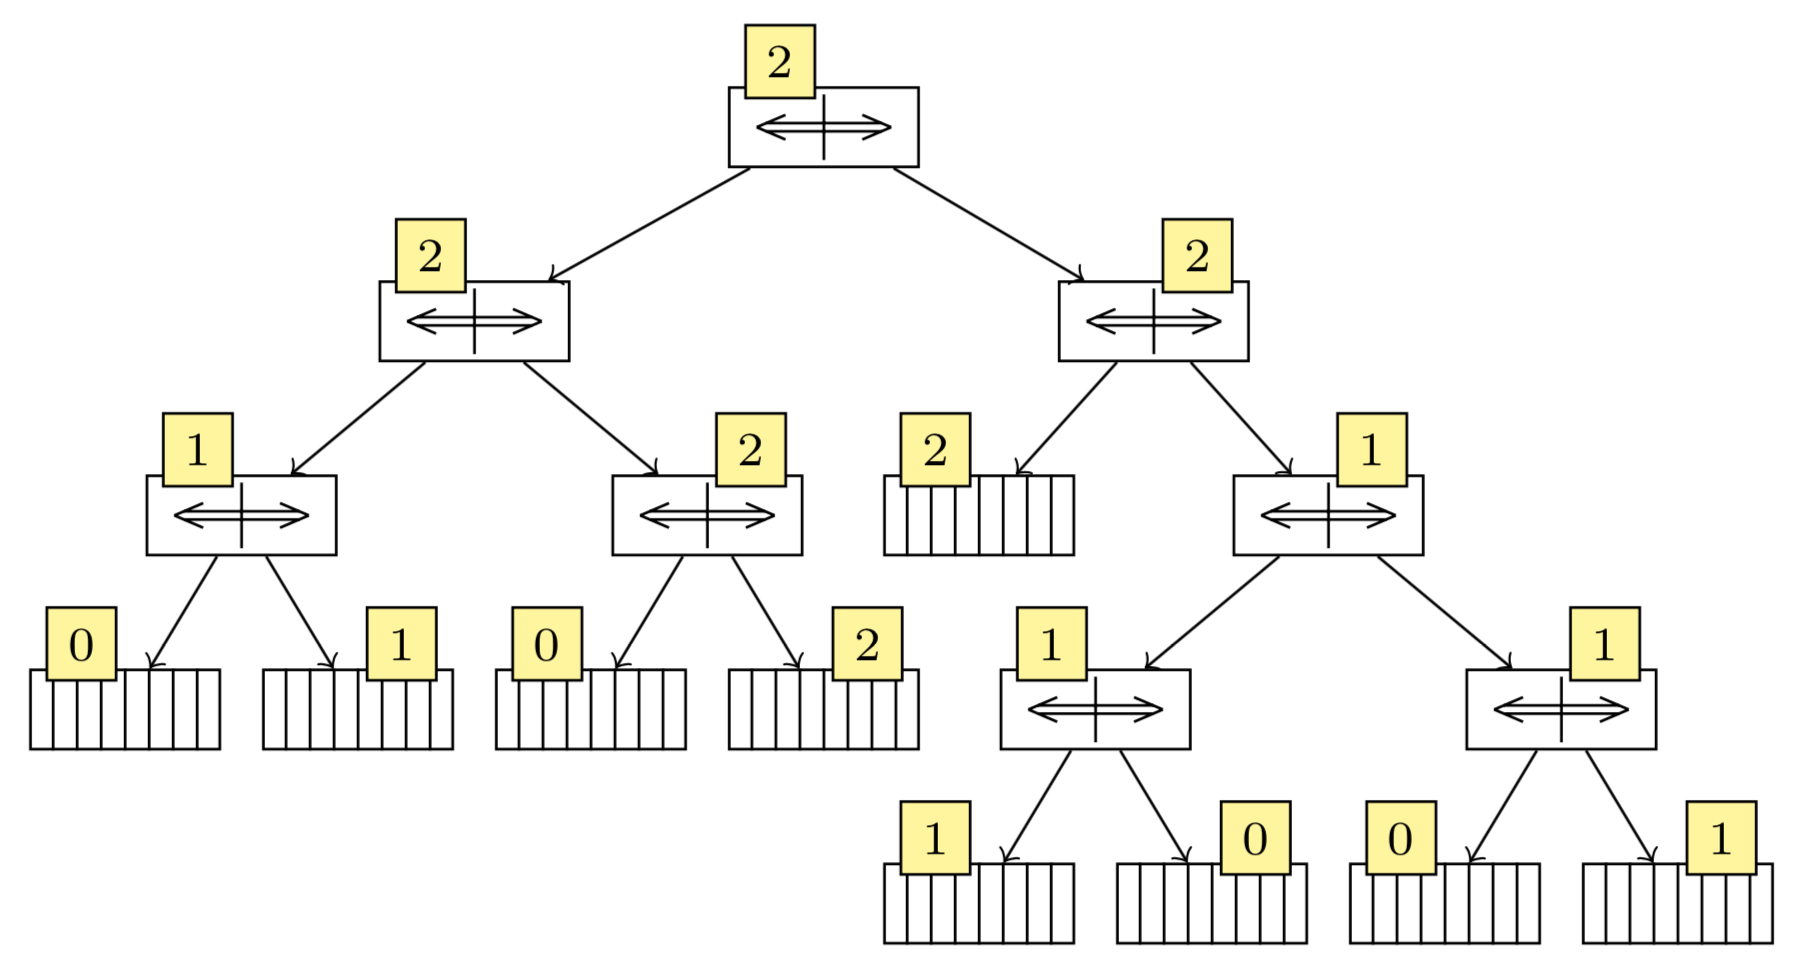
\includegraphics[width=15cm]{pic/ndtree_new.png}
\caption{Алгоритм ENS-NDT-ONE}.
\label{ndtree_new}
\end{center}
\end{figure}

В худшем случае алгоритм работает за $O(MN^2)$, аналогично оригинальному алгоритму ENS-NDT. Однако зачастую время работы алгоритма сильно лучше. Например, на случайно сгенерированных точках в гиперкубе $[0; 1]^M$, $O(N)$ точек с вероятностью более $1/2$ необходимо заходить в обоих детей в каждой не листовой вершине дерева. Таким образом получаем, верхняя граница асимптотики времени работы равна $O(MN^{1+log_2(3/2)}) \approx O(MN^{1.585})$.

\section{Анализ времени работы гибридного алгоритма}

В этом разделе дадим некоторую оценку асимптотики времени работы гибридного алгоритма.

We can now formulate the hybrid algorithm. We take the divide-and-conquer algorithm as a basis, however, before we enter the main parts of HelperA or HelperB, we check whether the subproblem is small enough. If it is, we use the ENS-NDT-ONE algorithm to solve this subproblem. Since ENS-NDT-ONE is immune to the features of these subproblems, such as the loss of monotonicity, the resulting algorithm will always produce correct results.

More formally, we define, for every number of objectives, a threshold which signifies that every subproblem with this number of objectives and the size below the threshold should be delegated to ENS-NDT-ONE. For HelperA, the size of the problem is the size of the set P, while for HelperB this is the sum of sizes of the sets L and R.

We shall note that, since we define thresholds to be constants, the asymp- totic estimation of the running time of this algorithm is still $O(N(\log N)^{M-1})$. However, we note that more careful choices for thresholds, that possibly depend on the number of objectives or on other properties of the subproblems, may possibly result in smaller runtime bounds. Due to the complexity of this issue, including heavy input dependency, we leave this for possible future work.


